% =====================================================================
%  EPD-SDIA-4112 -- Statistique Bayesienne -- Master 1 SDIA
%  CHAPITRE 3 : Estimation et inference bayesiennes (50 slides, 8 h)
%  Tous les nombres cites proviennent de src/fig_ch3.py et
%  src/fig_ch3b_pymc.py, reellement executes (figures/key_numbers_ch3.json).
% =====================================================================
\section{Chapitre 3 --- Estimation et inférence}

% ---------------------------------------------------------------- 1
\chapterslide{Chapitre 3}{Estimation et inférence bayésiennes}{8 h --- 5 sections --- 50 slides}{%
\textbf{Objectifs} --- passer du posterior à une \textbf{décision chiffrée} :
choisir un estimateur ponctuel justifié par une fonction de perte, construire et
interpréter un intervalle de crédibilité (queue égale, HDI, unilatéral),
prédire une observation future, et mesurer soi-même la couverture et le risque
par simulation.}

% ---------------------------------------------------------------- 2
\begin{frame}{Plan du chapitre 3 --- du posterior à la décision}
\footnotesize
\vspace{-2mm}
\begin{columns}[t]
\begin{column}{0.55\textwidth}
\begin{enumerate}
  \item[3.1] \textbf{Estimateurs ponctuels} et perte minimisée \hfill \textit{slides 3--16}
  \item[3.2] \textbf{Intervalles de crédibilité} : queue égale, HDI, unilatéral,
        comparaison rigoureuse avec l'IC fréquentiste \hfill \textit{slides 17--26}
  \item[3.3] \textbf{Prédiction a posteriori} et \textit{posterior predictive checks}
        \hfill \textit{slides 27--34}
  \item[3.4] \textbf{Cas appliqués} : Gamma-Poisson, Normal-Normal, régression
        bayésienne en PyMC, risque MSE \hfill \textit{slides 35--45}
  \item[3.5] \textbf{Synthèse, pièges et quiz} \hfill \textit{slides 46--50}
\end{enumerate}
\vspace{2mm}
\begin{tabular}{@{}llll@{}}
\toprule
\textbf{Volume} & \textbf{Cours} & \textbf{TD} & \textbf{TP machine} \\
\midrule
8 h & 5 h & 1 h 30 & 1 h 30 \\
\bottomrule
\end{tabular}
\end{column}
\begin{column}{0.43\textwidth}
\begin{kbox}[La question centrale]
On connaît $p(\theta \given y)$. On doit maintenant \textbf{livrer un chiffre} à un
décideur. Ce chiffre n'est pas unique : il dépend de \emph{ce que coûte une erreur}.
\vspace{1.5mm}

\small Trois sorties possibles : \warn{} un point, \warn{} un intervalle,
\warn{} une prédiction.
\end{kbox}
\end{column}
\end{columns}
\vspace{1mm}
\begin{tcolorbox}[colback=byCyan!8,colframe=byCyan,arc=2mm,width=.95\textwidth]
\centering\small
\textbf{Prérequis (chapitres 1--2)} : couples conjugués Beta-Binomial, Gamma-Poisson,
Normal-Normal ; loi a posteriori ; $n_0 = \alpha_0 + \beta_0$ comme « force du prior ».
\end{tcolorbox}
\end{frame}

% ---------------------------------------------------------------- 3
\begin{frame}{Section 3.1 --- Ce que « estimer » veut dire}
\begin{qbox}[QUIZ d'ouverture --- 4 min, vote à main levée]
Une étude donne $\mathrm{Beta}(3,7)$ comme loi a posteriori du taux de panne d'un
composant. On doit écrire \textbf{un seul nombre} dans le rapport technique.
\begin{enumerate}
  \item[(A)] $0{,}30$ (la moyenne)
  \item[(B)] $0{,}25$ (le mode)
  \item[(C)] la valeur qui minimise le coût moyen des erreurs \textbf{dans ce contexte}
  \item[(D)] n'importe laquelle : elles sont équivalentes
\end{enumerate}
\vspace{1.5mm}
\textbf{Réponse : (C).} La bonne question n'est pas « quelle est la valeur centrale ? »
mais « \emph{quelle erreur} est-ce que je paie ? ». On verra que (A) paie
$(\theta - a)^2$, (B) paie une perte 0--1, et que le posterior Beta$(3,7)$ donne
respectivement $0{,}300$, $0{,}286$ et $0{,}250$.
\end{qbox}
\vspace{1mm}
\begin{ebox}[Le glissement conceptuel de la séance]
Fréquentiste : « l'estimateur est \emph{bon} si sa loi d'échantillonnage
est centrée ». Bayésien : « l'estimateur est \emph{bon} si sa perte
attendue \textbf{sous le posterior} est minimale ».
\end{ebox}
\end{frame}

% ---------------------------------------------------------------- 4
\begin{frame}{Le risque a posteriori : la seule définition dont on a besoin}
\small
\vspace{-1mm}
\begin{kbox}[Définition --- risque a posteriori]
Soit $L(\theta, a)$ la perte subie quand on annonce $a$ alors que la vérité est $\theta$.
Le \textbf{risque a posteriori} de $a$ est
\[
\rho(a) \;=\; \E\big[\,L(\theta, a) \given y \,\big]
\;=\; \int L(\theta, a)\, p(\theta \given y)\,\mathrm{d}\theta .
\]
L'\textbf{estimateur bayésien} associé à la perte $L$ est
$\;a^\star = \argmin_{a} \rho(a)$.
\end{kbox}
\vspace{1mm}
\begin{columns}[t]
\begin{column}{0.53\textwidth}
\begin{ebox}[Trois remarques qui changent tout]
\begin{itemize}
  \item La perte $L$ est une \textbf{décision pédagogique}, pas une vérité
        mathématique : elle doit se justifier par le contexte.
  \item Le risque est calculé \textbf{sous le posterior}, donc il utilise les
        données \emph{et} le prior.
  \item $L$ peut être asymétrique : sous-estimer une crue n'est pas équivalent à
        la surestimer.
\end{itemize}
\end{ebox}
\end{column}
\begin{column}{0.45\textwidth}
\begin{tcolorbox}[colback=byLight,colframe=byGrey!55,arc=2mm]
\small\textbf{Perte asymétrique (exemple industriel)}
\[
L(\theta, a)=
\begin{cases}
c_- (a-\theta) & \text{si } a > \theta \\
c_+ (\theta-a) & \text{si } a < \theta
\end{cases}
\]
surstock \;/\; rupture. Avec $c_+ = 5 c_-$, l'optimum est
\textbf{un quantile}, pas la moyenne.
\end{tcolorbox}
\end{column}
\end{columns}
\end{frame}

% ---------------------------------------------------------------- 5
\begin{frame}{Trois pertes canoniques, trois estimateurs}
\begin{center}
{\small
\begin{tabular}{@{}p{0.16\textwidth}p{0.19\textwidth}p{0.18\textwidth}p{0.31\textwidth}@{}}
\toprule
\textbf{Perte} $L(\theta,a)$ & \textbf{Intuition} & \textbf{Estimateur} & \textbf{Quand l'utiliser} \\
\midrule
$(\theta-a)^2$ \newline quadratique & « une grosse erreur coûte très cher » &
\textbf{moyenne} $\E[\theta \given y]$ &
erreur symétrique, standard, résumés automatiques \\
\addlinespace
$|\theta-a|$ \newline absolue & « chaque unité d'écart coûte pareil » &
\textbf{médiane} du posterior &
données aberrantes, queues épaisses, HDI \\
\addlinespace
$\mathbf{1}\{|\theta-a| > \varepsilon\}$ \newline 0--1 & « seule compte la bonne
décision, à $\varepsilon$ près » &
\textbf{mode} (MAP) &
classification, seuil, décision binaire \\
\bottomrule
\end{tabular}}
\end{center}
\vspace{1.5mm}
\begin{ebox}[Le résultat à retenir par cœur]
\centering\small
quadratique $\rightarrow$ \textbf{moyenne} \quad$\vert$\quad
absolue $\rightarrow$ \textbf{médiane} \quad$\vert$\quad
0--1 $\rightarrow$ \textbf{mode} \;(\textit{maximum a posteriori})
\end{ebox}
\end{frame}

% ---------------------------------------------------------------- 6
\begin{frame}{Pourquoi ces trois-là ? Les calculs, en trois lignes}
\small
\vspace{-1.5mm}
\begin{ebox}[1. Perte quadratique $\Rightarrow$ la moyenne]
$\rho(a)=\E[(\theta-a)^2 \given y]$ se dérive en $a$ :
$\rho'(a) = -2\E[\theta \given y] + 2a$ ; en annulant, $\;a^\star = \E[\theta \given y]$.
La dérivée seconde vaut $2 > 0$ : c'est bien un minimum.
\end{ebox}
\vspace{1mm}
\begin{ebox}[2. Perte absolue $\Rightarrow$ la médiane]
$\rho(a)=\int |\theta-a| p(\theta \given y)\mathrm{d}\theta$ a pour dérivée
$\rho'(a) = P(\theta < a \given y) - P(\theta > a \given y)$ : elle s'annule
quand \textbf{autant de masse de chaque côté}, soit $a^\star = $ médiane.
\end{ebox}
\vspace{1mm}
\begin{ebox}[3. Perte 0--1 $\Rightarrow$ le mode]
$\rho(a) = 1 - \int_{a-\varepsilon}^{a+\varepsilon} p(\theta \given y)\mathrm{d}\theta$ :
minimiser la perte, c'est \textbf{maximiser la masse locale}. Pour un posterior
unimodal, l'optimum est le mode ; en général c'est le centre du plus petit
intervalle de masse $2\varepsilon$.
\end{ebox}
\vspace{1mm}
\begin{kbox}[Conséquence pratique]
La moyenne et la médiane \textbf{coïncident} si le posterior est symétrique.
Dès qu'il est asymétrique --- ce qui arrive à \emph{chaque fois que le prior ou la
vraisemblance penchent} --- les trois nombres divergent, et le choix devient une
décision.
\end{kbox}
\end{frame}

% ---------------------------------------------------------------- 7
\begin{frame}{Les trois estimateurs et leur perte, mesurés}
\begin{center}
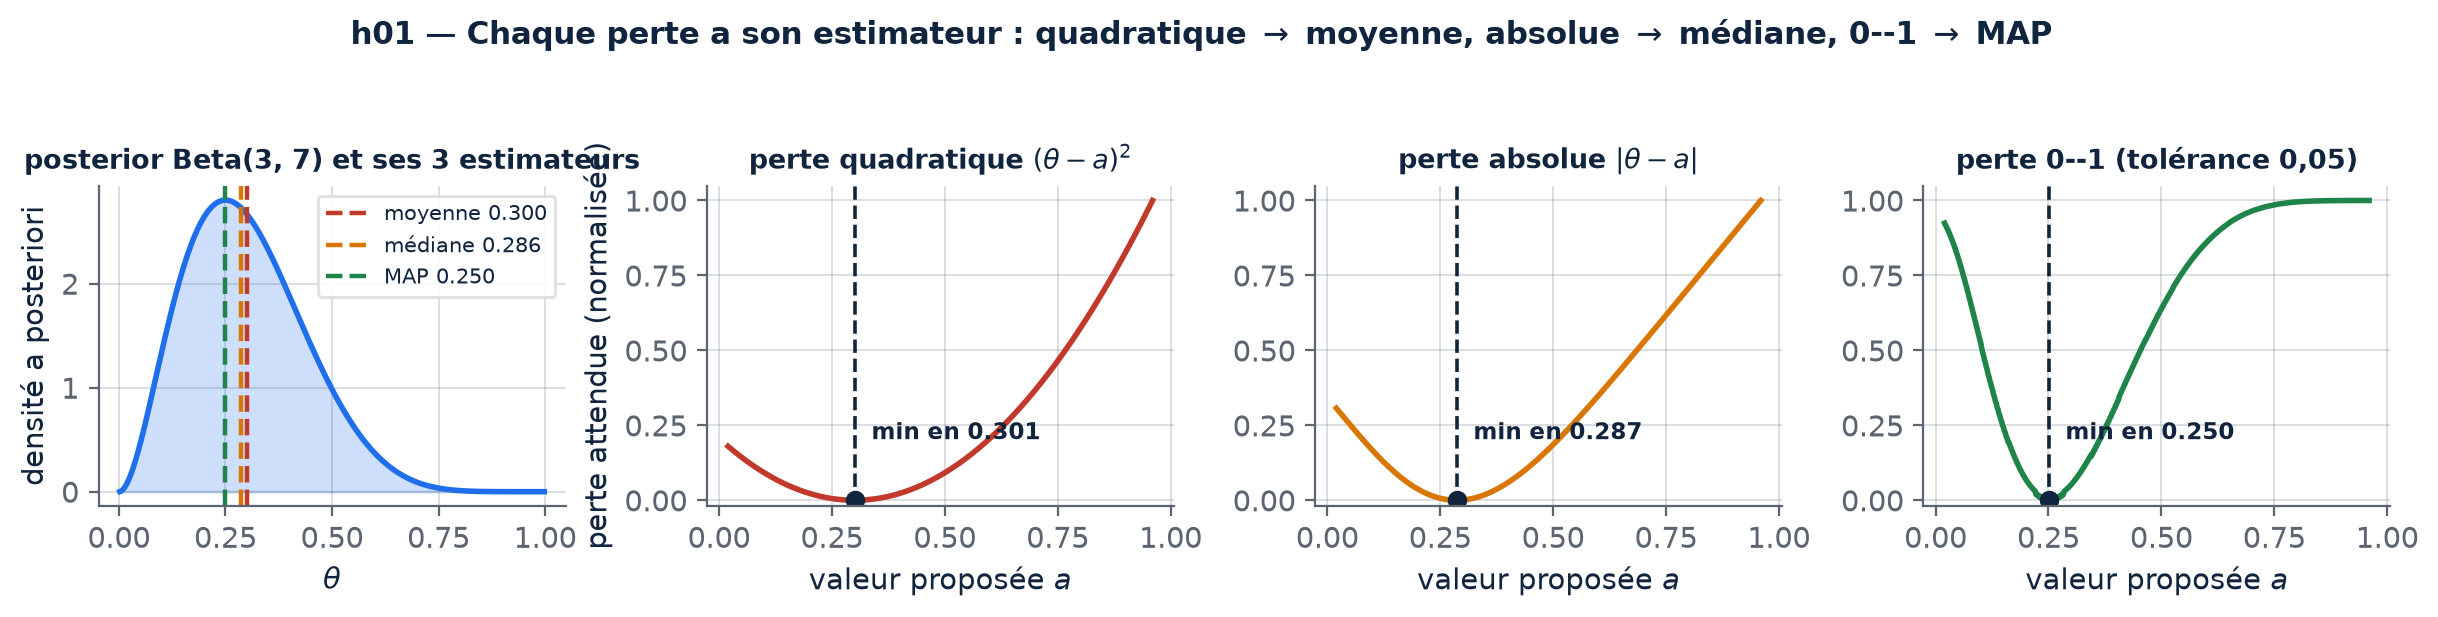
\includegraphics[width=.97\textwidth]{h01_estimateurs_pertes.png}
\end{center}
\vspace{-1mm}
\begin{columns}[t]
\begin{column}{0.55\textwidth}
\begin{ebox}[Lecture du graphique (calculs exécutés)]
Posterior \textbf{Beta$(3,7)$}, franchement asymétrique à droite. Les trois
pertes, évaluées sur une grille de $470$ valeurs de $a$, atteignent leur minimum
en trois points distincts : \textbf{la courbe de perte tranche, elle ne discute pas}.
\end{ebox}
\end{column}
\begin{column}{0.43\textwidth}
\begin{solbox}[Minima numériques trouvés]
\resizebox{\ifdim\width>\linewidth\linewidth\else\width\fi}{!}{%
\begin{tabular}{@{}lll@{}}
\toprule
Perte & $a^\star$ trouvé & estimateur \\
\midrule
quadratique & $0{,}301$ & moyenne $0{,}300$ \\
absolue & $0{,}287$ & médiane $0{,}286$ \\
0--1 ($\varepsilon{=}0{,}05$) & $0{,}250$ & mode $0{,}250$ \\
\bottomrule
\end{tabular}}
\vspace{1mm}

\tiny Écart mode -- moyenne : $0{,}050$ sur une échelle $[0\,;1]$, soit
$5$ points de taux : en industrie, ce n'est pas un détail.
\end{solbox}
\end{column}
\end{columns}
\end{frame}

% ---------------------------------------------------------------- 8
\begin{frame}{Tableau de bord : le posterior Beta$(3,7)$ en chiffres}
\small
\vspace{-1mm}
\begin{columns}[t]
\begin{column}{0.48\textwidth}
\begin{ebox}[Ce que la machine a calculé]
\begin{itemize}
  \item moyenne $\E[\theta \given y] = 0{,}300$
  \item médiane $= 0{,}286$
  \item mode (MAP) $= 0{,}250$
  \item $\argmin$ perte quadratique $= 0{,}301$
  \item $\argmin$ perte absolue $= 0{,}287$
  \item $\argmin$ perte 0--1 $= 0{,}250$
\end{itemize}
\vspace{1mm}
\footnotesize Les minima \emph{numériques} reproduisent les formules théoriques à
$0{,}001$ près : c'est la vérification qui doit être faite \textbf{avant} de faire
confiance à un code d'optimisation.
\end{ebox}
\end{column}
\begin{column}{0.50\textwidth}
\begin{kbox}[Le réflexe d'ingénieur]
\begin{enumerate}
  \item Calculer la moyenne (toujours possible, gratuite).
  \item Regarder l'\textbf{asymétrie} : si
        $\E[\theta \given y] \neq $ médiane, la moyenne est un choix, pas un dû.
  \item Demander au commanditaire : « que coûte une erreur de $+0{,}05$ ? et de $-0{,}05$ ? »
  \item Choisir l'estimateur, et \textbf{l'annoncer dans le rapport}.
\end{enumerate}
\end{kbox}
\end{column}
\end{columns}
\vspace{1mm}
\begin{wbox}[Ne jamais faire]
Rapporter la sortie par défaut de la librairie sans dire \textbf{de quelle perte}
elle correspond : \py{np.mean()} minimise l'erreur quadratique. Si le client paie
une perte absolue, vous n'avez pas optimisé \emph{son} problème.
\end{wbox}
\end{frame}

% ---------------------------------------------------------------- 9
\begin{frame}{Quiz --- Quelle perte pour quelle décision ?}
\begin{qbox}[Question 1 --- Rupture de stock]
Un magasin choisit la quantité $a$ à commander. Une rupture coûte cinq fois plus
qu'un invendu. La perte est
$L(\theta,a)=c|\theta-a|$ avec $c = 5$ si $a<\theta$, $c=1$ si $a>\theta$.
Quel résumé du posterior faut-il viser ?
\vspace{1.5mm}
\begin{enumerate}
  \item[(A)] la moyenne
  \item[(B)] la médiane
  \item[(C)] un \textbf{quantile supérieur} : $P(\theta \leq a \given y) \approx \frac{c_+}{c_+ + c_-}$
  \item[(D)] le mode
\end{enumerate}
\vspace{1mm}
\textbf{Réponse : (C).} La médiane correspondrait à $c_+ = c_-$. Le calcul de
$\rho'(a) = c_+ P(\theta > a \given y) - c_- P(\theta < a \given y)$ donne
$P(\theta > a \given y) = \frac{c_-}{c_+ + c_-} = \frac{1}{6}$, soit le
\textbf{quantile d'ordre $5/6 \approx 83{,}3\,\%$}.
\end{qbox}
\vspace{1mm}
\begin{kbox}[Le message]
\small Aucun estimateur n'est « bayésien » tout seul : \textbf{l'estimateur est
défini par la perte}. Changer la perte, c'est changer la réponse --- et c'est
exactement ce qu'on veut.
\end{kbox}
\end{frame}

% ---------------------------------------------------------------- 10
\begin{frame}{MAP contre maximum de vraisemblance}
\small
\vspace{-1mm}
\begin{columns}[t]
\begin{column}{0.52\textwidth}
\begin{kbox}[Deux arguments, à un terme près]
\[
\text{MAP} = \argmax_\theta \; \underbrace{p(\theta \given y)}_{\propto\, p(y \given \theta) p(\theta)}
\qquad\qquad
\text{MLE} = \argmax_\theta \; p(y \given \theta)
\]
En passant au logarithme :
\[
\log p(\theta \given y) = \log p(y \given \theta) + \log p(\theta) + \text{cste}.
\]
Le prior n'est donc rien d'autre qu'une \textbf{pénalité} ajoutée à la
log-vraisemblance --- ce que les statisticiens appellent une régularisation.
\end{kbox}
\end{column}
\begin{column}{0.46\textwidth}
\begin{ebox}[Lecture moderne]
\begin{itemize}
  \item Prior uniforme $\Rightarrow$ MAP $=$ MLE.
  \item Prior $\N(0, \tau^2)$ $\Rightarrow$ pénalité $\ell_2$
        (crête / \textit{ridge}).
  \item Prior Laplace $\Rightarrow$ pénalité $\ell_1$
        (lasso, parcimonie).
  \item Prior Beta$(\alpha_0, \beta_0)$ $\Rightarrow$ moyenne a posteriori
        $=$ compteur de succès et d'échecs \textbf{ajoutés} aux données.
\end{itemize}
\end{ebox}
\end{column}
\end{columns}
\vspace{1mm}
\begin{wbox}[La différence de fond avec le MLE]
Le MLE est \textbf{invariant} par reparamétrisation ($\hat\theta$ et $g(\hat\theta)$ se correspondent). Le MAP
n'est \textbf{pas} invariant : changer de paramètre change le prior, donc change
le mode. \textbf{La moyenne a posteriori}, elle, se transforme correctement.
\end{wbox}
\end{frame}

% ---------------------------------------------------------------- 11
\begin{frame}{Exemple chiffré : Beta-Bernoulli, $k = 14$ succès sur $n = 20$}
\begin{columns}[t]
\begin{column}{0.47\textwidth}
\begin{ebox}[Les deux estimateurs, en formules]
\small
Avec $n_0 = \alpha_0 + \beta_0$ et $m_0 = \alpha_0/n_0$ :
\[
\hat\theta_{\text{MLE}} = \frac{k}{n} = \frac{14}{20} = 0{,}700
\]
\[
\theta_{\text{MAP}} = \frac{k + \alpha_0 - 1}{n + \alpha_0 + \beta_0 - 2}
\]
\[
\E[\theta \given y] = \frac{k + \alpha_0}{n + \alpha_0 + \beta_0}
= \frac{k + n_0 m_0}{n + n_0}
\]
\end{ebox}
\end{column}
\begin{column}{0.51\textwidth}
\begin{solbox}[Prior centré sur $0{,}40$]
\resizebox{\ifdim\width>\linewidth\linewidth\else\width\fi}{!}{%
\begin{tabular}{@{}lccc@{}}
\toprule
Force du prior & moyenne a post. & MAP & poids des données \\
\midrule
$n_0 = 2$   & $0{,}673$ & $0{,}690$ & $0{,}909$ \\
$n_0 = 10$  & $0{,}600$ & $0{,}607$ & $0{,}667$ \\
$n_0 = 100$ & $0{,}450$ & $0{,}449$ & $0{,}167$ \\
\midrule
\multicolumn{4}{@{}l@{}}{\textbf{MLE (le prior est ignoré)} : $0{,}700$} \\
\bottomrule
\end{tabular}}
\vspace{1.5mm}

\small Le poids des données est $\frac{n}{n+n_0}$ : c'est la \textbf{formule de la
moyenne pondérée} entre ce que disent les données et ce que dit le prior.
\end{solbox}
\end{column}
\end{columns}
\vspace{1mm}
\begin{abox}[Exercice éclair (3 min, en binôme)]
Avec $n = 20$, $k = 14$ et un prior centré sur $0{,}40$ : quel $n_0$ rend données
et prior équipondérés, et quelle est alors la moyenne a posteriori ?
\vspace{0.5mm}

\textbf{Réponse :} $n_0 = n = 20$ ($w = 0{,}5$) et
$0{,}5 \times 0{,}70 + 0{,}5 \times 0{,}40 = 0{,}55$.
\end{abox}
\end{frame}

% ---------------------------------------------------------------- 12
\begin{frame}{Visualiser le \textit{shrinkage} : le MAP est tiré vers le prior}
\small
\vspace{-1.5mm}
\begin{center}
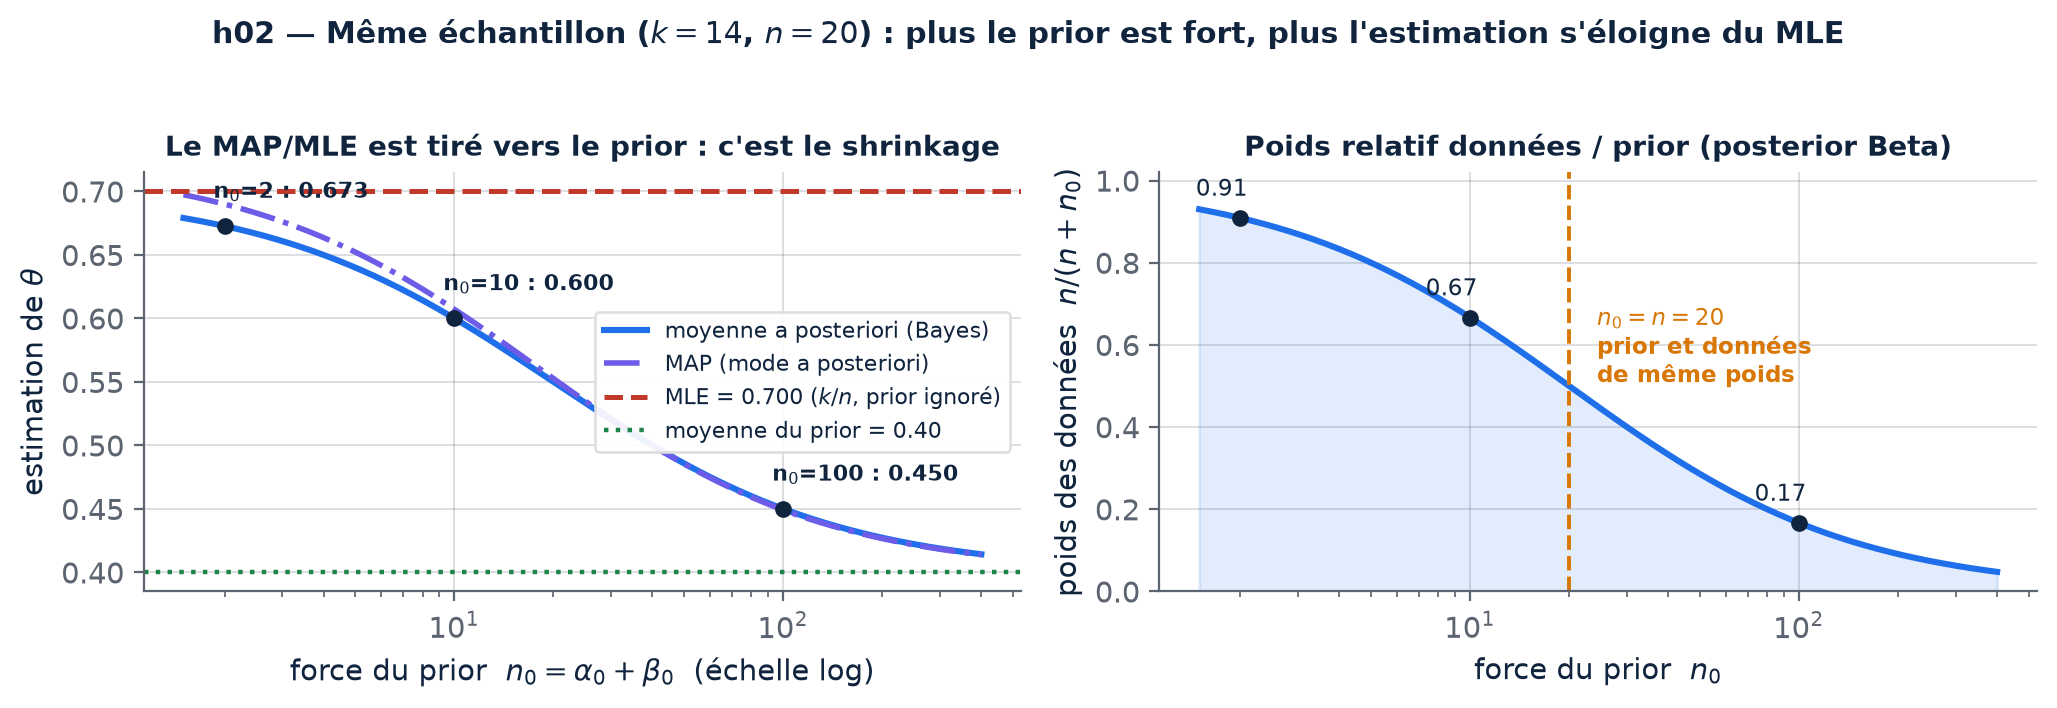
\includegraphics[width=.84\textwidth]{h02_shrinkage_prior.png}
\end{center}
\vspace{-1.5mm}
\begin{columns}[t]
\begin{column}{0.62\textwidth}
\begin{ebox}[Ce que montrent les deux panneaux]
Le MLE vaut $0{,}700$ et ne bouge jamais. La moyenne a posteriori et le MAP
s'en écartent d'autant plus que le prior est fort, et \textbf{convergent} vers
$0{,}700$ quand $n_0 \to 0$. Pour $n_0 = n = 20$, prior et données pèsent
exactement pareil : la moyenne tombe à mi-chemin entre $0{,}40$ et $0{,}70$.
\end{ebox}
\end{column}
\begin{column}{0.36\textwidth}
\begin{kbox}[Shrinkage]
Le terme anglais signifie « rétraction » : l'estimation est
\textbf{rétractée} vers le centre du prior. Ce n'est pas un défaut de méthode,
c'est exactement ce qui \textbf{réduit le risque} aux petits échantillons
(section 3.4, figure du MSE).
\end{kbox}
\end{column}
\end{columns}
\end{frame}

% ---------------------------------------------------------------- 13
\begin{frame}{Biais, variance et shrinkage : le vrai mécanisme}
\begin{columns}[t]
\begin{column}{0.49\textwidth}
\begin{ebox}[Décomposition biais--variance (fréquentiste)]
Pour $\hat\theta$ estimant $\theta$ :
\[
\E[(\hat\theta - \theta)^2]
= \underbrace{\big(\E[\hat\theta] - \theta\big)^2}_{\text{biais}^2}
+ \underbrace{\Var(\hat\theta)}_{\text{variance}} .
\]
Le MLE est \textbf{sans biais} mais de variance $\frac{\theta(1-\theta)}{n}$.
La moyenne a posteriori est \textbf{biaisée} (vers la croyance a priori) mais de
variance plus faible : le compromis peut améliorer le MSE total.
\end{ebox}
\end{column}
\begin{column}{0.49\textwidth}
\begin{solbox}[MSE mesuré : 500 simulations]
\resizebox{\ifdim\width>\linewidth\linewidth\else\width\fi}{!}{%
\begin{tabular}{@{}lccc@{}}
\toprule
$n$ & MSE (MLE) & MSE (Bayes) & rapport \\
\midrule
$5$   & $0{,}04526$ & $0{,}01853$ & $\mathbf{0{,}41}$ \\
$20$  & --- & --- & $0{,}74$ \\
$400$ & $0{,}000518$ & $0{,}000518$ & $1{,}00$ \\
\bottomrule
\end{tabular}}
\vspace{1.5mm}
\tiny Aux petits échantillons, le bayésien divise le risque par $\approx 2{,}4$ ;
à $n = 400$, l'avantage disparaît : \textbf{les données prennent le pouvoir}.
\end{solbox}
\end{column}
\end{columns}
\vspace{1mm}
\begin{kbox}[La formule du compromis, en une ligne]
La moyenne a posteriori est un \textbf{estimateur rétréci} :
$a^\star = w\,\hat\theta_{\text{MLE}} + (1-w)\, m_0$ avec $w = \frac{n}{n+n_0}$.
Optimiser $w$ revient à optimiser le compromis biais--variance.
\end{kbox}
\end{frame}

% ---------------------------------------------------------------- 14
\begin{frame}{Activité guidée --- 8 minutes, par binômes}
\begin{abox}[Énoncé]
Un posterior est $\mathrm{Beta}(3, 7)$. On dispose de Python et de
\file{scipy.stats}.
\begin{enumerate}
  \item Calculez \textbf{à la main} la moyenne, la médiane et le mode.
  \item Retrouvez-les avec \py{stats.beta(3,7).mean()} et
        \py{stats.beta(3,7).median()}.
  \item Écrivez une boucle qui évalue $\rho(a)$ pour les trois pertes sur
        \py{a} de $0{,}02$ à $0{,}96$, et vérifiez les minima trouvés.
  \item \textbf{Question subsidiaire} : pour quelle valeur de $c_+/c_-$ la
        perte absolue asymétrique du slide 4 donne-t-elle exactement la moyenne ?
\end{enumerate}
\end{abox}
\vspace{1mm}
\begin{columns}[t]
\begin{column}{0.49\textwidth}
\begin{solbox}[Résultats attendus (vérifiés par le script du cours)]
moyenne $0{,}300$, médiane $0{,}286$, mode $0{,}250$ ;
minima numériques $0{,}301$, $0{,}287$, $0{,}250$.
\end{solbox}
\end{column}
\begin{column}{0.49\textwidth}
\begin{kbox}[Subsidiaire, la réponse]
Non : avec $c_+ = c_-$ on retombe sur la médiane. Pour obtenir la moyenne, il
faut une perte quadratique : une pénalité qui croît avec le \emph{carré} de
l'écart, et non linéairement.
\end{kbox}
\end{column}
\end{columns}
\end{frame}

% ---------------------------------------------------------------- 15
\begin{frame}{Synthèse de la section 3.1}
\begin{center}
{\small
\begin{tabular}{@{}p{0.16\textwidth}p{0.14\textwidth}p{0.12\textwidth}p{0.40\textwidth}@{}}
\toprule
\textbf{Perte} & \textbf{Estimateur} & \textbf{symboles} & \textbf{Propriétés / précautions} \\
\midrule
quadratique $(\theta-a)^2$ & moyenne & $\E[\theta \given y]$ &
toujours définie, se transforme bien ; sensible aux queues épaisses \\
\addlinespace
absolue $|\theta-a|$ & médiane & $q_{0{,}5}$ &
robuste ; cohérente avec le HDI ; pas de formule fermée simple \\
\addlinespace
0--1 & mode (MAP) & $\argmax p(\theta \given y)$ &
lien direct avec le MLE et la régularisation ; \textbf{non invariant} par
reparamétrisation \\
\addlinespace
asymétrique & quantile & $q_{\,c_+/(c_++c_-)}$ &
traduit les coûts réels du métier (rupture, crue, fraude) \\
\bottomrule
\end{tabular}}
\end{center}
\vspace{1.5mm}
\begin{kbox}[À retenir en une phrase]
Un estimateur ponctuel n'est pas « la réponse » : c'est \textbf{la réponse à une
question de coût}. Le posterior est le même pour tous ; seule la perte change.
\end{kbox}
\end{frame}

% ---------------------------------------------------------------- 16
\begin{frame}{Section 3.2 --- Du point à l'intervalle : trois constructions}
\small
\vspace{-1mm}
\begin{columns}[t]
\begin{column}{0.31\textwidth}
\begin{ebox}[1. Queues égales]
On coupe $2{,}5\,\%$ de masse de chaque côté :
$[q_{0{,}025}\,;\,q_{0{,}975}]$.

\vspace{1mm}\footnotesize Valeur par défaut : une ligne de code, se résume bien.
\end{ebox}
\end{column}
\begin{column}{0.31\textwidth}
\begin{ebox}[2. HDI (densité postérieure la plus élevée)]
L'intervalle \textbf{le plus court} de masse $0{,}95$ : chaque point dedans a une
densité supérieure à chaque point dehors.

\vspace{1mm}\footnotesize Indispensable pour les posteriors fortement asymétriques
(Gamma, Beta extrêmes).
\end{ebox}
\end{column}
\begin{column}{0.33\textwidth}
\begin{ebox}[3. Unilatéral]
\scriptsize
Le seuil $\theta_0$ est-il dépassé ? On annonce
$q_{5\%}$ et $P(\theta > \theta_0 \given y)$.

\vspace{1mm} Répond à une question de décision.
\end{ebox}
\end{column}
\end{columns}
\vspace{-0.5mm}
\begin{kbox}[Définition d'un intervalle de crédibilité de niveau $1-\alpha$]
Tout ensemble $C \subset \Theta$ tel que
\[
P(\theta \in C \given y) = \int_C p(\theta \given y)\,\mathrm{d}\theta = 1-\alpha .
\]
Il n'y a donc \emph{pas unicité} : le choix des bornes est une décision
supplémentaire.
\end{kbox}
\end{frame}

% ---------------------------------------------------------------- 17
\begin{frame}{HDI contre queues égales : le plus court gagne}
\small
\vspace{-2mm}
\begin{center}
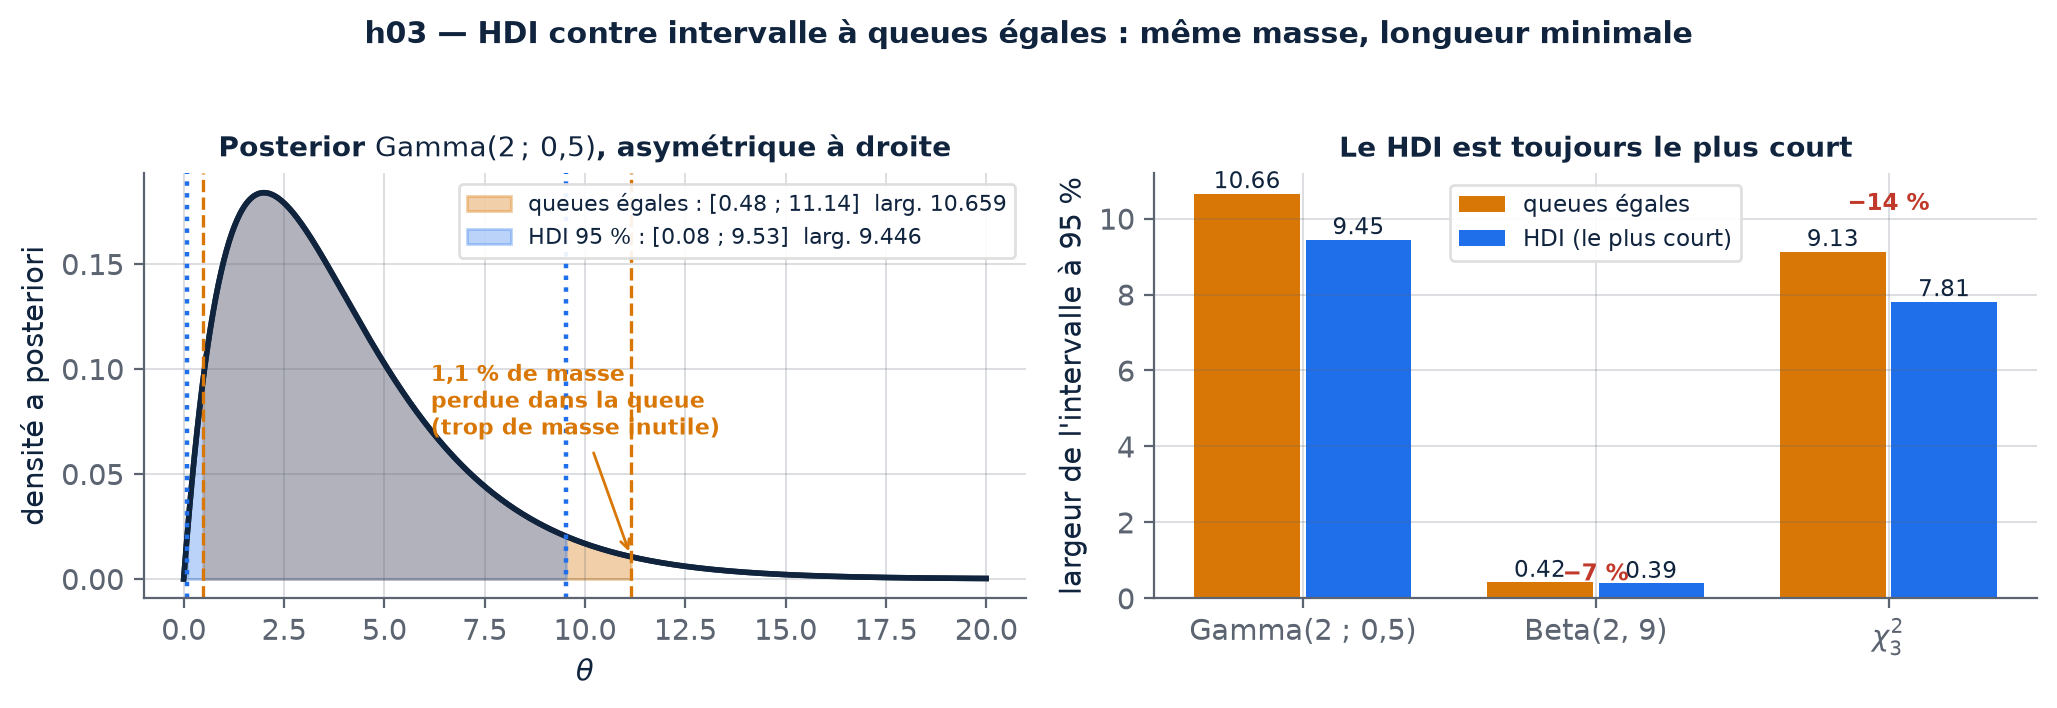
\includegraphics[width=.80\textwidth]{h03_hdi_vs_queue.png}
\end{center}
\vspace{-2.5mm}
\begin{columns}[t]
\begin{column}{0.56\textwidth}
\begin{ebox}[Calculs exécutés sur trois posteriors asymétriques]
\small
\begin{tabular}{@{}lccc@{}}
\toprule
Posterior & queues égales & HDI 95 \% & gain \\
\midrule
Gamma$(2\,;\,0{,}5)$ & $[0{,}484\,;\,11{,}143]$ & $[0{,}080\,;\,9{,}526]$ & $-11{,}4\,\%$ \\
Beta$(2,9)$ & largeur $0{,}4198$ & largeur $0{,}3905$ & $-7{,}0\,\%$ \\
$\chi^2_3$ & largeur $9{,}133$ & largeur $7{,}814$ & $-14{,}4\,\%$ \\
\bottomrule
\end{tabular}
\end{ebox}
\end{column}
\begin{column}{0.42\textwidth}
\begin{kbox}[Pourquoi l'écart existe]
L'intervalle à queues égales coupe \textbf{en probabilité} ($2{,}5\,\%$ de chaque
côté), pas \textbf{en densité}. Sur une loi à queue droite épaisse, il garde des
valeurs très improbables à droite pour satisfaire la symétrie de masse.
Le HDI, lui, coupe là où la densité est égale : sa largeur est minimale.
\end{kbox}
\end{column}
\end{columns}
\end{frame}
\nb{50}
